\documentclass[1p]{elsarticle_modified}
%\bibliographystyle{elsarticle-num}

%\usepackage[colorlinks]{hyperref}
%\usepackage{abbrmath_seonhwa} %\Abb, \Ascr, \Acal ,\Abf, \Afrak
\usepackage{amsfonts}
\usepackage{amssymb}
\usepackage{amsmath}
\usepackage{amsthm}
\usepackage{scalefnt}
\usepackage{amsbsy}
\usepackage{kotex}
\usepackage{caption}
\usepackage{subfig}
\usepackage{color}
\usepackage{graphicx}
\usepackage{xcolor} %% white, black, red, green, blue, cyan, magenta, yellow
\usepackage{float}
\usepackage{setspace}
\usepackage{hyperref}

\usepackage{tikz}
\usetikzlibrary{arrows}

\usepackage{multirow}
\usepackage{array} % fixed length table
\usepackage{hhline}

%%%%%%%%%%%%%%%%%%%%%
\makeatletter
\renewcommand*\env@matrix[1][\arraystretch]{%
	\edef\arraystretch{#1}%
	\hskip -\arraycolsep
	\let\@ifnextchar\new@ifnextchar
	\array{*\c@MaxMatrixCols c}}
\makeatother %https://tex.stackexchange.com/questions/14071/how-can-i-increase-the-line-spacing-in-a-matrix
%%%%%%%%%%%%%%%

\usepackage[normalem]{ulem}

\newcommand{\msout}[1]{\ifmmode\text{\sout{\ensuremath{#1}}}\else\sout{#1}\fi}
%SOURCE: \msout is \stkout macro in https://tex.stackexchange.com/questions/20609/strikeout-in-math-mode

\newcommand{\cancel}[1]{
	\ifmmode
	{\color{red}\msout{#1}}
	\else
	{\color{red}\sout{#1}}
	\fi
}

\newcommand{\add}[1]{
	{\color{blue}\uwave{#1}}
}

\newcommand{\replace}[2]{
	\ifmmode
	{\color{red}\msout{#1}}{\color{blue}\uwave{#2}}
	\else
	{\color{red}\sout{#1}}{\color{blue}\uwave{#2}}
	\fi
}

\newcommand{\Sol}{\mathcal{S}} %segment
\newcommand{\D}{D} %diagram
\newcommand{\A}{\mathcal{A}} %arc


%%%%%%%%%%%%%%%%%%%%%%%%%%%%%5 test

\def\sl{\operatorname{\textup{SL}}(2,\Cbb)}
\def\psl{\operatorname{\textup{PSL}}(2,\Cbb)}
\def\quan{\mkern 1mu \triangleright \mkern 1mu}

\theoremstyle{definition}
\newtheorem{thm}{Theorem}[section]
\newtheorem{prop}[thm]{Proposition}
\newtheorem{lem}[thm]{Lemma}
\newtheorem{ques}[thm]{Question}
\newtheorem{cor}[thm]{Corollary}
\newtheorem{defn}[thm]{Definition}
\newtheorem{exam}[thm]{Example}
\newtheorem{rmk}[thm]{Remark}
\newtheorem{alg}[thm]{Algorithm}

\newcommand{\I}{\sqrt{-1}}
\begin{document}

%\begin{frontmatter}
%
%\title{Boundary parabolic representations of knots up to 8 crossings}
%
%%% Group authors per affiliation:
%\author{Yunhi Cho} 
%\address{Department of Mathematics, University of Seoul, Seoul, Korea}
%\ead{yhcho@uos.ac.kr}
%
%
%\author{Seonhwa Kim} %\fnref{s_kim}}
%\address{Center for Geometry and Physics, Institute for Basic Science, Pohang, 37673, Korea}
%\ead{ryeona17@ibs.re.kr}
%
%\author{Hyuk Kim}
%\address{Department of Mathematical Sciences, Seoul National University, Seoul 08826, Korea}
%\ead{hyukkim@snu.ac.kr}
%
%\author{Seokbeom Yoon}
%\address{Department of Mathematical Sciences, Seoul National University, Seoul, 08826,  Korea}
%\ead{sbyoon15@snu.ac.kr}
%
%\begin{abstract}
%We find all boundary parabolic representation of knots up to 8 crossings.
%
%\end{abstract}
%\begin{keyword}
%    \MSC[2010] 57M25 
%\end{keyword}
%
%\end{frontmatter}

%\linenumbers
%\tableofcontents
%
\newcommand\colored[1]{\textcolor{white}{\rule[-0.35ex]{0.8em}{1.4ex}}\kern-0.8em\color{red} #1}%
%\newcommand\colored[1]{\textcolor{white}{ #1}\kern-2.17ex	\textcolor{white}{ #1}\kern-1.81ex	\textcolor{white}{ #1}\kern-2.15ex\color{red}#1	}

{\Large $\underline{12n_{0258}~(K12n_{0258})}$}

\setlength{\tabcolsep}{10pt}
\renewcommand{\arraystretch}{1.6}
\vspace{1cm}\begin{tabular}{m{100pt}>{\centering\arraybackslash}m{274pt}}
\multirow{5}{120pt}{
	\centering
	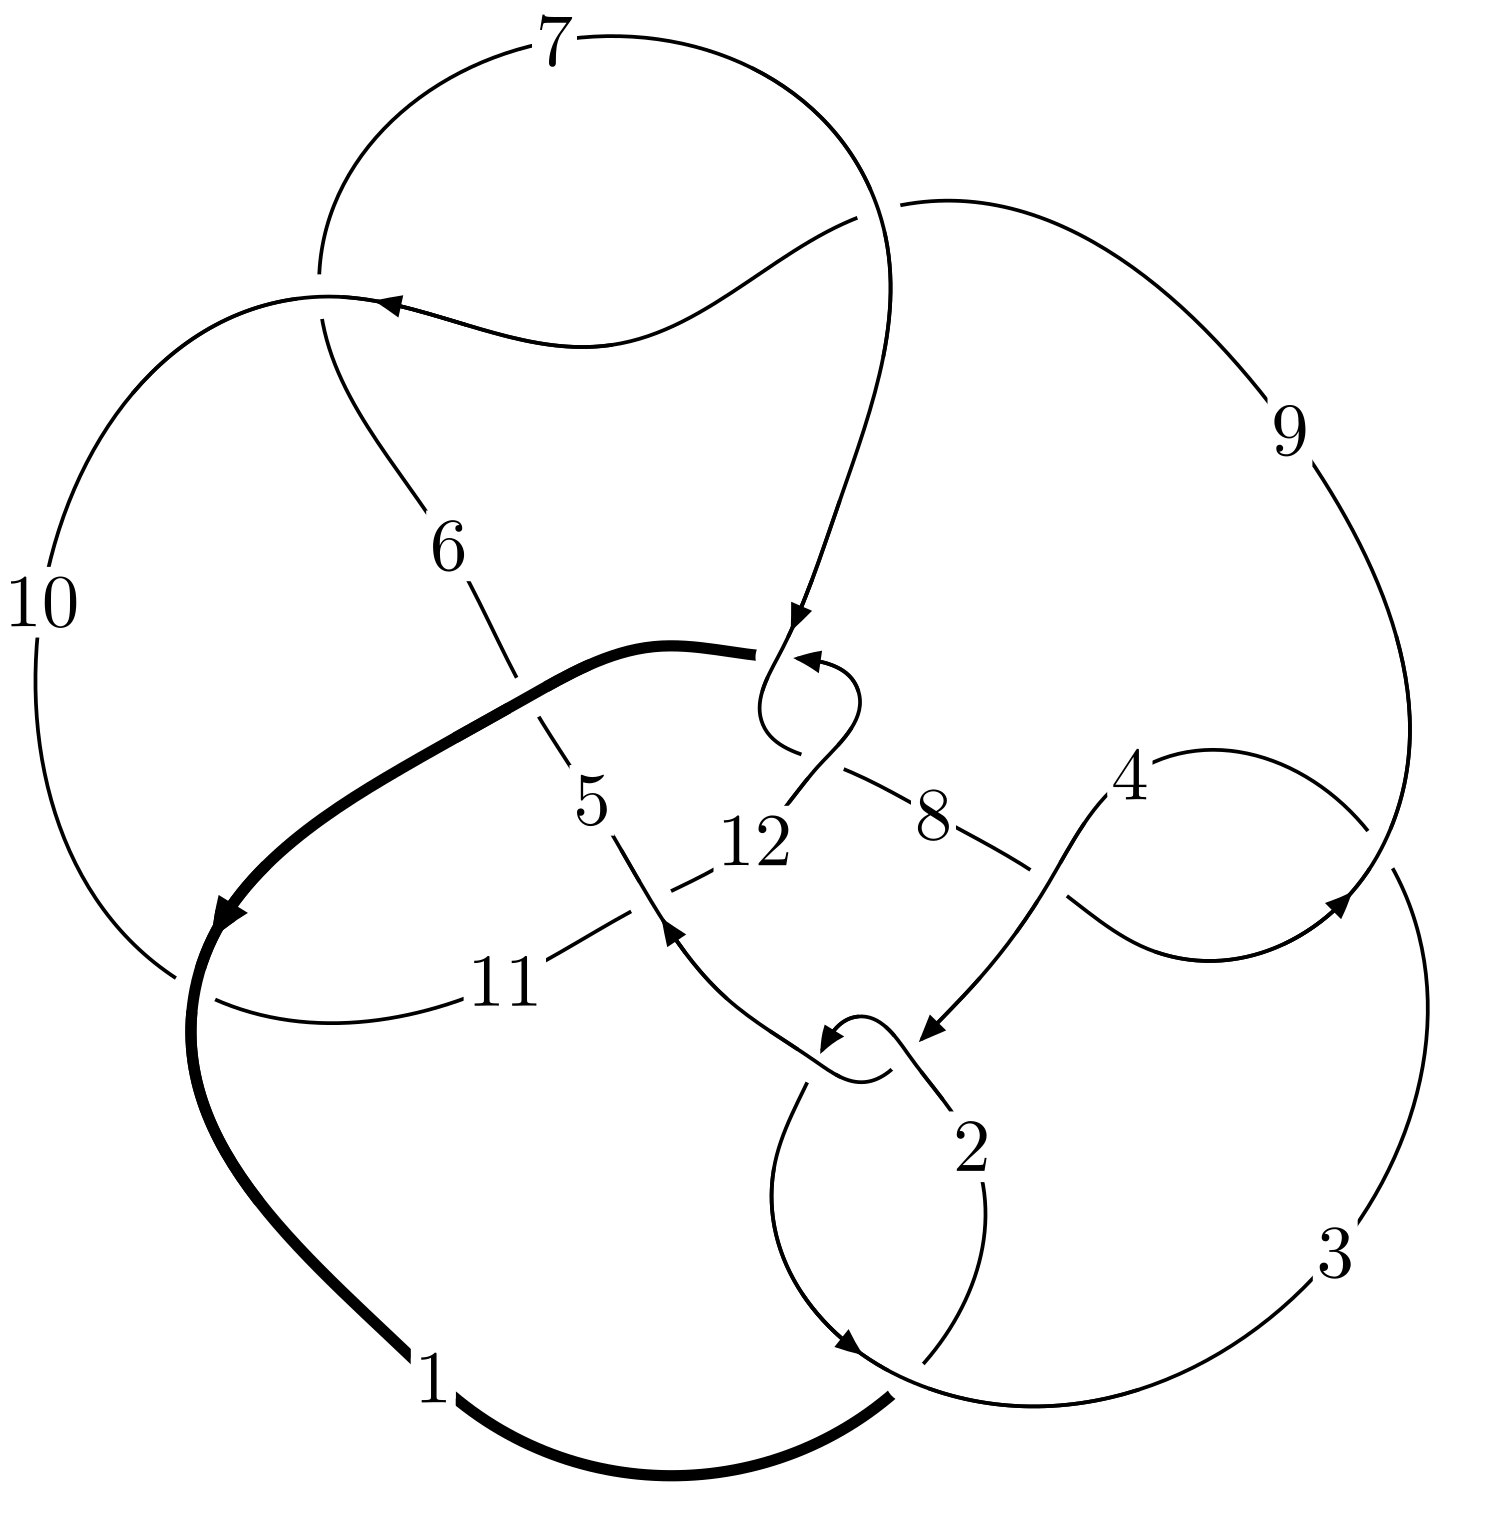
\includegraphics[width=112pt]{../../../GIT/diagram.site/Diagrams/png/2347_12n_0258.png}\\
\ \ \ A knot diagram\footnotemark}&
\allowdisplaybreaks
\textbf{Linearized knot diagam} \\
\cline{2-2}
 &
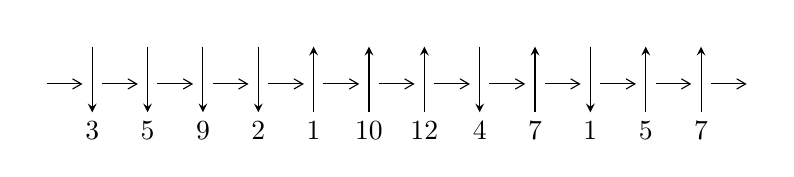
\begin{tikzpicture}[x=20pt, y=17pt]
	% nodes
	\node (C0) at (0, 0) {};
	\node (C1) at (1, 0) {};
	\node (C1U) at (1, +1) {};
	\node (C1D) at (1, -1) {3};

	\node (C2) at (2, 0) {};
	\node (C2U) at (2, +1) {};
	\node (C2D) at (2, -1) {5};

	\node (C3) at (3, 0) {};
	\node (C3U) at (3, +1) {};
	\node (C3D) at (3, -1) {9};

	\node (C4) at (4, 0) {};
	\node (C4U) at (4, +1) {};
	\node (C4D) at (4, -1) {2};

	\node (C5) at (5, 0) {};
	\node (C5U) at (5, +1) {};
	\node (C5D) at (5, -1) {1};

	\node (C6) at (6, 0) {};
	\node (C6U) at (6, +1) {};
	\node (C6D) at (6, -1) {10};

	\node (C7) at (7, 0) {};
	\node (C7U) at (7, +1) {};
	\node (C7D) at (7, -1) {12};

	\node (C8) at (8, 0) {};
	\node (C8U) at (8, +1) {};
	\node (C8D) at (8, -1) {4};

	\node (C9) at (9, 0) {};
	\node (C9U) at (9, +1) {};
	\node (C9D) at (9, -1) {7};

	\node (C10) at (10, 0) {};
	\node (C10U) at (10, +1) {};
	\node (C10D) at (10, -1) {1};

	\node (C11) at (11, 0) {};
	\node (C11U) at (11, +1) {};
	\node (C11D) at (11, -1) {5};

	\node (C12) at (12, 0) {};
	\node (C12U) at (12, +1) {};
	\node (C12D) at (12, -1) {7};
	\node (C13) at (13, 0) {};

	% arrows
	\draw[->,>={angle 60}]
	(C0) edge (C1) (C1) edge (C2) (C2) edge (C3) (C3) edge (C4) (C4) edge (C5) (C5) edge (C6) (C6) edge (C7) (C7) edge (C8) (C8) edge (C9) (C9) edge (C10) (C10) edge (C11) (C11) edge (C12) (C12) edge (C13) ;	\draw[->,>=stealth]
	(C1U) edge (C1D) (C2U) edge (C2D) (C3U) edge (C3D) (C4U) edge (C4D) (C5D) edge (C5U) (C6D) edge (C6U) (C7D) edge (C7U) (C8U) edge (C8D) (C9D) edge (C9U) (C10U) edge (C10D) (C11D) edge (C11U) (C12D) edge (C12U) ;
	\end{tikzpicture} \\
\hhline{~~} \\& 
\textbf{Solving Sequence} \\ \cline{2-2} 
 &
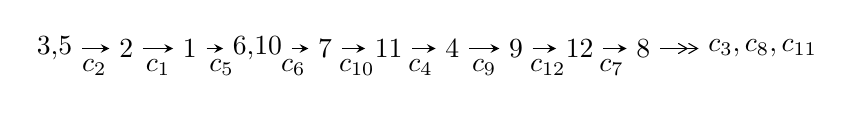
\begin{tikzpicture}[x=23pt, y=7pt]
	% node
	\node (A0) at (-1/8, 0) {3,5};
	\node (A1) at (1, 0) {2};
	\node (A2) at (2, 0) {1};
	\node (A3) at (49/16, 0) {6,10};
	\node (A4) at (33/8, 0) {7};
	\node (A5) at (41/8, 0) {11};
	\node (A6) at (49/8, 0) {4};
	\node (A7) at (57/8, 0) {9};
	\node (A8) at (65/8, 0) {12};
	\node (A9) at (73/8, 0) {8};
	\node (C1) at (1/2, -1) {$c_{2}$};
	\node (C2) at (3/2, -1) {$c_{1}$};
	\node (C3) at (5/2, -1) {$c_{5}$};
	\node (C4) at (29/8, -1) {$c_{6}$};
	\node (C5) at (37/8, -1) {$c_{10}$};
	\node (C6) at (45/8, -1) {$c_{4}$};
	\node (C7) at (53/8, -1) {$c_{9}$};
	\node (C8) at (61/8, -1) {$c_{12}$};
	\node (C9) at (69/8, -1) {$c_{7}$};
	\node (A10) at (11, 0) {$c_{3},c_{8},c_{11}$};

	% edge
	\draw[->,>=stealth]	
	(A0) edge (A1) (A1) edge (A2) (A2) edge (A3) (A3) edge (A4) (A4) edge (A5) (A5) edge (A6) (A6) edge (A7) (A7) edge (A8) (A8) edge (A9) ;
	\draw[->>,>={angle 60}]	
	(A9) edge (A10);
\end{tikzpicture} \\ 

\end{tabular} \\

\footnotetext{
The image of knot diagram is generated by the software ``\textbf{Draw programme}" developed by Andrew Bartholomew(\url{http://www.layer8.co.uk/maths/draw/index.htm\#Running-draw}), where we modified some parts for our purpose(\url{https://github.com/CATsTAILs/LinksPainter}).
}\phantom \\ \newline 
\centering \textbf{Ideals for irreducible components\footnotemark of $X_{\text{par}}$} 
 
\begin{align*}
I^u_{1}&=\langle 
102949 u^{15}+169425 u^{14}+\cdots+344734 b-488230,\\
\phantom{I^u_{1}}&\phantom{= \langle  }475025 u^{15}+757448 u^{14}+\cdots+689468 a-2984519,\;u^{16}+2 u^{15}+\cdots-15 u-4\rangle \\
I^u_{2}&=\langle 
u^5 a+2 u^4 a+u^5+4 u^4-2 u^2 a+3 u^3-2 a u-2 u^2+3 b-2 a-3 u-1,\;4 u^4-2 u^2 a- u^3+a^2-7 u^2+2 a+5,\\
\phantom{I^u_{2}}&\phantom{= \langle  }u^6+u^5- u^4-2 u^3+u+1\rangle \\
I^u_{3}&=\langle 
a u+b+u+1,\;a^2+a u+3,\;u^2+u-1\rangle \\
I^u_{4}&=\langle 
2 b+1,\;a-1,\;u-1\rangle \\
\\
\end{align*}
\raggedright * 4 irreducible components of $\dim_{\mathbb{C}}=0$, with total 33 representations.\\
\footnotetext{All coefficients of polynomials are rational numbers. But the coefficients are sometimes approximated in decimal forms when there is not enough margin.}
\newpage
\renewcommand{\arraystretch}{1}
\centering \section*{I. $I^u_{1}= \langle 1.03\times10^{5} u^{15}+1.69\times10^{5} u^{14}+\cdots+3.45\times10^{5} b-4.88\times10^{5},\;4.75\times10^{5} u^{15}+7.57\times10^{5} u^{14}+\cdots+6.89\times10^{5} a-2.98\times10^{6},\;u^{16}+2 u^{15}+\cdots-15 u-4 \rangle$}
\flushleft \textbf{(i) Arc colorings}\\
\begin{tabular}{m{7pt} m{180pt} m{7pt} m{180pt} }
\flushright $a_{3}=$&$\begin{pmatrix}1\\0\end{pmatrix}$ \\
\flushright $a_{5}=$&$\begin{pmatrix}0\\u\end{pmatrix}$ \\
\flushright $a_{2}=$&$\begin{pmatrix}1\\- u^2\end{pmatrix}$ \\
\flushright $a_{1}=$&$\begin{pmatrix}- u^2+1\\- u^2\end{pmatrix}$ \\
\flushright $a_{6}=$&$\begin{pmatrix}u^5-2 u^3+u\\u^5- u^3+u\end{pmatrix}$ \\
\flushright $a_{10}=$&$\begin{pmatrix}-0.688973 u^{15}-1.09860 u^{14}+\cdots+10.8060 u+4.32873\\-0.298633 u^{15}-0.491466 u^{14}+\cdots+4.30076 u+1.41625\end{pmatrix}$ \\
\flushright $a_{7}=$&$\begin{pmatrix}0.527611 u^{15}+0.764711 u^{14}+\cdots-7.10340 u-2.57154\\0.0757251 u^{15}+0.157434 u^{14}+\cdots-0.695406 u-0.399317\end{pmatrix}$ \\
\flushright $a_{11}=$&$\begin{pmatrix}-0.396324 u^{15}-0.532866 u^{14}+\cdots+5.76866 u+2.60958\\-0.296495 u^{15}-0.408933 u^{14}+\cdots+4.60606 u+1.80754\end{pmatrix}$ \\
\flushright $a_{4}=$&$\begin{pmatrix}u\\- u^3+u\end{pmatrix}$ \\
\flushright $a_{9}=$&$\begin{pmatrix}-1.08530 u^{15}-1.63146 u^{14}+\cdots+16.5746 u+5.93830\\-0.447127 u^{15}-0.705112 u^{14}+\cdots+6.59538 u+2.18466\end{pmatrix}$ \\
\flushright $a_{12}=$&$\begin{pmatrix}-0.396324 u^{15}-0.532866 u^{14}+\cdots+5.76866 u+2.60958\\-0.148494 u^{15}-0.213646 u^{14}+\cdots+2.29462 u+0.768413\end{pmatrix}$ \\
\flushright $a_{8}=$&$\begin{pmatrix}0.896155 u^{15}+1.26037 u^{14}+\cdots-12.0524 u-4.14979\\0.122193 u^{15}+0.231518 u^{14}+\cdots-1.42447 u-0.424931\end{pmatrix}$\\&\end{tabular}
\flushleft \textbf{(ii) Obstruction class $= -1$}\\~\\
\flushleft \textbf{(iii) Cusp Shapes $= \frac{2007761}{689468} u^{15}+\frac{2194435}{689468} u^{14}+\cdots-\frac{28351265}{689468} u-\frac{1282717}{172367}$}\\~\\
\newpage\renewcommand{\arraystretch}{1}
\flushleft \textbf{(iv) u-Polynomials at the component}\newline \\
\begin{tabular}{m{50pt}|m{274pt}}
Crossings & \hspace{64pt}u-Polynomials at each crossing \\
\hline $$\begin{aligned}c_{1}\end{aligned}$$&$\begin{aligned}
&u^{16}+10 u^{15}+\cdots+65 u+16
\end{aligned}$\\
\hline $$\begin{aligned}c_{2},c_{4}\end{aligned}$$&$\begin{aligned}
&u^{16}-2 u^{15}+\cdots+15 u-4
\end{aligned}$\\
\hline $$\begin{aligned}c_{3},c_{8}\end{aligned}$$&$\begin{aligned}
&u^{16}-3 u^{15}+\cdots+6 u+8
\end{aligned}$\\
\hline $$\begin{aligned}c_{5}\end{aligned}$$&$\begin{aligned}
&u^{16}-3 u^{15}+\cdots+52 u+64
\end{aligned}$\\
\hline $$\begin{aligned}c_{6},c_{7},c_{9}\\c_{11},c_{12}\end{aligned}$$&$\begin{aligned}
&u^{16}- u^{15}+\cdots- u-1
\end{aligned}$\\
\hline $$\begin{aligned}c_{10}\end{aligned}$$&$\begin{aligned}
&u^{16}-12 u^{15}+\cdots-50 u+4
\end{aligned}$\\
\hline
\end{tabular}\\~\\
\newpage\renewcommand{\arraystretch}{1}
\flushleft \textbf{(v) Riley Polynomials at the component}\newline \\
\begin{tabular}{m{50pt}|m{274pt}}
Crossings & \hspace{64pt}Riley Polynomials at each crossing \\
\hline $$\begin{aligned}c_{1}\end{aligned}$$&$\begin{aligned}
&y^{16}-6 y^{15}+\cdots+1343 y+256
\end{aligned}$\\
\hline $$\begin{aligned}c_{2},c_{4}\end{aligned}$$&$\begin{aligned}
&y^{16}-10 y^{15}+\cdots-65 y+16
\end{aligned}$\\
\hline $$\begin{aligned}c_{3},c_{8}\end{aligned}$$&$\begin{aligned}
&y^{16}+3 y^{15}+\cdots-52 y+64
\end{aligned}$\\
\hline $$\begin{aligned}c_{5}\end{aligned}$$&$\begin{aligned}
&y^{16}+67 y^{15}+\cdots-140304 y+4096
\end{aligned}$\\
\hline $$\begin{aligned}c_{6},c_{7},c_{9}\\c_{11},c_{12}\end{aligned}$$&$\begin{aligned}
&y^{16}+31 y^{15}+\cdots-9 y+1
\end{aligned}$\\
\hline $$\begin{aligned}c_{10}\end{aligned}$$&$\begin{aligned}
&y^{16}-36 y^{15}+\cdots-2908 y+16
\end{aligned}$\\
\hline
\end{tabular}\\~\\
\newpage\flushleft \textbf{(vi) Complex Volumes and Cusp Shapes}
$$\begin{array}{c|c|c}  
\text{Solutions to }I^u_{1}& \I (\text{vol} + \sqrt{-1}CS) & \text{Cusp shape}\\
 \hline 
\begin{aligned}
u &= \phantom{-}0.891782\phantom{ +0.000000I} \\
a &= \phantom{-}0.236674\phantom{ +0.000000I} \\
b &= -0.553091\phantom{ +0.000000I}\end{aligned}
 & -1.30085\phantom{ +0.000000I} & -8.84520\phantom{ +0.000000I} \\ \hline\begin{aligned}
u &= \phantom{-}1.091810 + 0.330825 I \\
a &= -0.147665 + 0.051010 I \\
b &= \phantom{-}0.210193 - 0.600885 I\end{aligned}
 & -3.22144 - 1.13355 I & -4.59977 + 1.25337 I \\ \hline\begin{aligned}
u &= \phantom{-}1.091810 - 0.330825 I \\
a &= -0.147665 - 0.051010 I \\
b &= \phantom{-}0.210193 + 0.600885 I\end{aligned}
 & -3.22144 + 1.13355 I & -4.59977 - 1.25337 I \\ \hline\begin{aligned}
u &= -1.094020 + 0.526074 I \\
a &= -1.054950 - 0.663309 I \\
b &= \phantom{-}0.141861 - 0.569038 I\end{aligned}
 & -1.87639 + 6.13504 I & \phantom{-}0.06427 - 7.98576 I \\ \hline\begin{aligned}
u &= -1.094020 - 0.526074 I \\
a &= -1.054950 + 0.663309 I \\
b &= \phantom{-}0.141861 + 0.569038 I\end{aligned}
 & -1.87639 - 6.13504 I & \phantom{-}0.06427 + 7.98576 I \\ \hline\begin{aligned}
u &= -0.029850 + 1.272860 I \\
a &= \phantom{-}4.37033 - 0.53285 I \\
b &= \phantom{-}3.61404 - 0.37068 I\end{aligned}
 & \phantom{-}19.7225 - 4.8173 I & -2.30205 + 1.82839 I \\ \hline\begin{aligned}
u &= -0.029850 - 1.272860 I \\
a &= \phantom{-}4.37033 + 0.53285 I \\
b &= \phantom{-}3.61404 + 0.37068 I\end{aligned}
 & \phantom{-}19.7225 + 4.8173 I & -2.30205 - 1.82839 I \\ \hline\begin{aligned}
u &= -1.31580\phantom{ +0.000000I} \\
a &= \phantom{-}0.254567\phantom{ +0.000000I} \\
b &= -1.49207\phantom{ +0.000000I}\end{aligned}
 & -0.940295\phantom{ +0.000000I} & -7.17020\phantom{ +0.000000I} \\ \hline\begin{aligned}
u &= -0.296508 + 0.600916 I \\
a &= \phantom{-}0.432297 - 1.059770 I \\
b &= -0.140186 - 0.553162 I\end{aligned}
 & \phantom{-}0.34157 - 1.65330 I & \phantom{-}2.57923 + 4.74775 I \\ \hline\begin{aligned}
u &= -0.296508 - 0.600916 I \\
a &= \phantom{-}0.432297 + 1.059770 I \\
b &= -0.140186 + 0.553162 I\end{aligned}
 & \phantom{-}0.34157 + 1.65330 I & \phantom{-}2.57923 - 4.74775 I\\
 \hline 
 \end{array}$$\newpage$$\begin{array}{c|c|c}  
\text{Solutions to }I^u_{1}& \I (\text{vol} + \sqrt{-1}CS) & \text{Cusp shape}\\
 \hline 
\begin{aligned}
u &= -0.537130 + 0.286418 I \\
a &= \phantom{-}0.60885 + 1.51474 I \\
b &= -0.016541 + 0.547073 I\end{aligned}
 & \phantom{-}0.96164 + 1.16578 I & \phantom{-}5.62628 - 5.26913 I \\ \hline\begin{aligned}
u &= -0.537130 - 0.286418 I \\
a &= \phantom{-}0.60885 - 1.51474 I \\
b &= -0.016541 - 0.547073 I\end{aligned}
 & \phantom{-}0.96164 - 1.16578 I & \phantom{-}5.62628 + 5.26913 I \\ \hline\begin{aligned}
u &= -1.42350 + 0.64934 I \\
a &= -1.89897 + 2.53374 I \\
b &= -3.64218 + 0.84571 I\end{aligned}
 & \phantom{-}15.4087 + 11.5569 I & -4.10768 - 4.68861 I \\ \hline\begin{aligned}
u &= -1.42350 - 0.64934 I \\
a &= -1.89897 - 2.53374 I \\
b &= -3.64218 - 0.84571 I\end{aligned}
 & \phantom{-}15.4087 - 11.5569 I & -4.10768 + 4.68861 I \\ \hline\begin{aligned}
u &= \phantom{-}1.50121 + 0.66208 I \\
a &= -1.43051 - 3.06754 I \\
b &= -3.39461 - 1.98308 I\end{aligned}
 & \phantom{-}15.0197 - 2.0565 I & -4.37753 + 0.79044 I \\ \hline\begin{aligned}
u &= \phantom{-}1.50121 - 0.66208 I \\
a &= -1.43051 + 3.06754 I \\
b &= -3.39461 + 1.98308 I\end{aligned}
 & \phantom{-}15.0197 + 2.0565 I & -4.37753 - 0.79044 I\\
 \hline 
 \end{array}$$\newpage\newpage\renewcommand{\arraystretch}{1}
\centering \section*{II. $I^u_{2}= \langle u^5 a+u^5+\cdots-2 a-1,\;4 u^4-2 u^2 a- u^3+a^2-7 u^2+2 a+5,\;u^6+u^5- u^4-2 u^3+u+1 \rangle$}
\flushleft \textbf{(i) Arc colorings}\\
\begin{tabular}{m{7pt} m{180pt} m{7pt} m{180pt} }
\flushright $a_{3}=$&$\begin{pmatrix}1\\0\end{pmatrix}$ \\
\flushright $a_{5}=$&$\begin{pmatrix}0\\u\end{pmatrix}$ \\
\flushright $a_{2}=$&$\begin{pmatrix}1\\- u^2\end{pmatrix}$ \\
\flushright $a_{1}=$&$\begin{pmatrix}- u^2+1\\- u^2\end{pmatrix}$ \\
\flushright $a_{6}=$&$\begin{pmatrix}u^5-2 u^3+u\\u^5- u^3+u\end{pmatrix}$ \\
\flushright $a_{10}=$&$\begin{pmatrix}a\\-\frac{1}{3} u^5 a-\frac{1}{3} u^5+\cdots+\frac{2}{3} a+\frac{1}{3}\end{pmatrix}$ \\
\flushright $a_{7}=$&$\begin{pmatrix}\frac{1}{3} u^5 a+\frac{4}{3} u^5+\cdots+\frac{1}{3} a+\frac{5}{3}\\-\frac{1}{3} u^5 a+\frac{2}{3} u^5+\cdots+\frac{2}{3} a+\frac{1}{3}\end{pmatrix}$ \\
\flushright $a_{11}=$&$\begin{pmatrix}\frac{1}{3} u^4 a+\frac{1}{3} u^5+\cdots+\frac{2}{3} a+1\\-\frac{2}{3} u^5 a-\frac{2}{3} u^4 a+\cdots+\frac{2}{3} a+\frac{2}{3}\end{pmatrix}$ \\
\flushright $a_{4}=$&$\begin{pmatrix}u\\- u^3+u\end{pmatrix}$ \\
\flushright $a_{9}=$&$\begin{pmatrix}-\frac{1}{3} u^4 a-\frac{1}{3} u^5+\cdots+\frac{1}{3} a-\frac{2}{3} u\\\frac{1}{3} u^4 a-\frac{2}{3} u^5+\cdots-\frac{1}{3} a-\frac{1}{3} u\end{pmatrix}$ \\
\flushright $a_{12}=$&$\begin{pmatrix}\frac{1}{3} u^4 a+\frac{1}{3} u^5+\cdots+\frac{2}{3} a+1\\-\frac{1}{3} u^5 a+\frac{1}{3} u^5+\cdots+a+\frac{1}{3}\end{pmatrix}$ \\
\flushright $a_{8}=$&$\begin{pmatrix}\frac{1}{3} u^5 a+\frac{1}{3} u^5+\cdots+\frac{1}{3} a+\frac{2}{3}\\\frac{2}{3} u^5 a+\frac{2}{3} u^4 a+\cdots+\frac{1}{3} a+\frac{1}{3}\end{pmatrix}$\\&\end{tabular}
\flushleft \textbf{(ii) Obstruction class $= 1$}\\~\\
\flushleft \textbf{(iii) Cusp Shapes $= 4 u^4-4 u^2-4 u-4$}\\~\\
\newpage\renewcommand{\arraystretch}{1}
\flushleft \textbf{(iv) u-Polynomials at the component}\newline \\
\begin{tabular}{m{50pt}|m{274pt}}
Crossings & \hspace{64pt}u-Polynomials at each crossing \\
\hline $$\begin{aligned}c_{1},c_{5}\end{aligned}$$&$\begin{aligned}
&(u^6-3 u^5+5 u^4-4 u^3+2 u^2- u+1)^2
\end{aligned}$\\
\hline $$\begin{aligned}c_{2}\end{aligned}$$&$\begin{aligned}
&(u^6+u^5- u^4-2 u^3+u+1)^2
\end{aligned}$\\
\hline $$\begin{aligned}c_{3},c_{8}\end{aligned}$$&$\begin{aligned}
&u^{12}+3 u^{10}+5 u^8+4 u^6+2 u^4+u^2+1
\end{aligned}$\\
\hline $$\begin{aligned}c_{4}\end{aligned}$$&$\begin{aligned}
&(u^6- u^5- u^4+2 u^3- u+1)^2
\end{aligned}$\\
\hline $$\begin{aligned}c_{6},c_{7},c_{9}\\c_{11},c_{12}\end{aligned}$$&$\begin{aligned}
&(u^2+1)^6
\end{aligned}$\\
\hline $$\begin{aligned}c_{10}\end{aligned}$$&$\begin{aligned}
&u^{12}-12 u^{11}+\cdots-60 u+9
\end{aligned}$\\
\hline
\end{tabular}\\~\\
\newpage\renewcommand{\arraystretch}{1}
\flushleft \textbf{(v) Riley Polynomials at the component}\newline \\
\begin{tabular}{m{50pt}|m{274pt}}
Crossings & \hspace{64pt}Riley Polynomials at each crossing \\
\hline $$\begin{aligned}c_{1},c_{5}\end{aligned}$$&$\begin{aligned}
&(y^6+y^5+5 y^4+6 y^2+3 y+1)^2
\end{aligned}$\\
\hline $$\begin{aligned}c_{2},c_{4}\end{aligned}$$&$\begin{aligned}
&(y^6-3 y^5+5 y^4-4 y^3+2 y^2- y+1)^2
\end{aligned}$\\
\hline $$\begin{aligned}c_{3},c_{8}\end{aligned}$$&$\begin{aligned}
&(y^6+3 y^5+5 y^4+4 y^3+2 y^2+y+1)^2
\end{aligned}$\\
\hline $$\begin{aligned}c_{6},c_{7},c_{9}\\c_{11},c_{12}\end{aligned}$$&$\begin{aligned}
&(y+1)^{12}
\end{aligned}$\\
\hline $$\begin{aligned}c_{10}\end{aligned}$$&$\begin{aligned}
&y^{12}-14 y^{11}+\cdots-108 y+81
\end{aligned}$\\
\hline
\end{tabular}\\~\\
\newpage\flushleft \textbf{(vi) Complex Volumes and Cusp Shapes}
$$\begin{array}{c|c|c}  
\text{Solutions to }I^u_{2}& \I (\text{vol} + \sqrt{-1}CS) & \text{Cusp shape}\\
 \hline 
\begin{aligned}
u &= \phantom{-}1.002190 + 0.295542 I \\
a &= \phantom{-}0.387926 + 1.194620 I \\
b &= \phantom{-}1.74846 - 0.37806 I\end{aligned}
 & -5.18047 - 0.92430 I & -9.71672 + 0.79423 I \\ \hline\begin{aligned}
u &= \phantom{-}1.002190 + 0.295542 I \\
a &= -0.553835 - 0.009862 I \\
b &= -0.37806 - 1.74846 I\end{aligned}
 & -5.18047 - 0.92430 I & -9.71672 + 0.79423 I \\ \hline\begin{aligned}
u &= \phantom{-}1.002190 - 0.295542 I \\
a &= \phantom{-}0.387926 - 1.194620 I \\
b &= \phantom{-}1.74846 + 0.37806 I\end{aligned}
 & -5.18047 + 0.92430 I & -9.71672 - 0.79423 I \\ \hline\begin{aligned}
u &= \phantom{-}1.002190 - 0.295542 I \\
a &= -0.553835 + 0.009862 I \\
b &= -0.37806 + 1.74846 I\end{aligned}
 & -5.18047 + 0.92430 I & -9.71672 - 0.79423 I \\ \hline\begin{aligned}
u &= -0.428243 + 0.664531 I \\
a &= -2.09808 + 1.60703 I \\
b &= -1.188690 + 0.647273 I\end{aligned}
 & -1.39926 - 0.92430 I & -2.28328 + 0.79423 I \\ \hline\begin{aligned}
u &= -0.428243 + 0.664531 I \\
a &= -0.41834 - 2.74535 I \\
b &= -0.647273 - 1.188690 I\end{aligned}
 & -1.39926 - 0.92430 I & -2.28328 + 0.79423 I \\ \hline\begin{aligned}
u &= -0.428243 - 0.664531 I \\
a &= -2.09808 - 1.60703 I \\
b &= -1.188690 - 0.647273 I\end{aligned}
 & -1.39926 + 0.92430 I & -2.28328 - 0.79423 I \\ \hline\begin{aligned}
u &= -0.428243 - 0.664531 I \\
a &= -0.41834 + 2.74535 I \\
b &= -0.647273 + 1.188690 I\end{aligned}
 & -1.39926 + 0.92430 I & -2.28328 - 0.79423 I \\ \hline\begin{aligned}
u &= -1.073950 + 0.558752 I \\
a &= \phantom{-}1.42256 - 0.62619 I \\
b &= \phantom{-}1.114040 + 0.351534 I\end{aligned}
 & -3.28987 + 5.69302 I & -6.00000 - 5.51057 I \\ \hline\begin{aligned}
u &= -1.073950 + 0.558752 I \\
a &= -1.74023 - 1.77409 I \\
b &= \phantom{-}0.351534 - 1.114040 I\end{aligned}
 & -3.28987 + 5.69302 I & -6.00000 - 5.51057 I\\
 \hline 
 \end{array}$$\newpage$$\begin{array}{c|c|c}  
\text{Solutions to }I^u_{2}& \I (\text{vol} + \sqrt{-1}CS) & \text{Cusp shape}\\
 \hline 
\begin{aligned}
u &= -1.073950 - 0.558752 I \\
a &= \phantom{-}1.42256 + 0.62619 I \\
b &= \phantom{-}1.114040 - 0.351534 I\end{aligned}
 & -3.28987 - 5.69302 I & -6.00000 + 5.51057 I \\ \hline\begin{aligned}
u &= -1.073950 - 0.558752 I \\
a &= -1.74023 + 1.77409 I \\
b &= \phantom{-}0.351534 + 1.114040 I\end{aligned}
 & -3.28987 - 5.69302 I & -6.00000 + 5.51057 I\\
 \hline 
 \end{array}$$\newpage\newpage\renewcommand{\arraystretch}{1}
\centering \section*{III. $I^u_{3}= \langle a u+b+u+1,\;a^2+a u+3,\;u^2+u-1 \rangle$}
\flushleft \textbf{(i) Arc colorings}\\
\begin{tabular}{m{7pt} m{180pt} m{7pt} m{180pt} }
\flushright $a_{3}=$&$\begin{pmatrix}1\\0\end{pmatrix}$ \\
\flushright $a_{5}=$&$\begin{pmatrix}0\\u\end{pmatrix}$ \\
\flushright $a_{2}=$&$\begin{pmatrix}1\\u-1\end{pmatrix}$ \\
\flushright $a_{1}=$&$\begin{pmatrix}u\\u-1\end{pmatrix}$ \\
\flushright $a_{6}=$&$\begin{pmatrix}2 u-1\\4 u-2\end{pmatrix}$ \\
\flushright $a_{10}=$&$\begin{pmatrix}a\\- a u- u-1\end{pmatrix}$ \\
\flushright $a_{7}=$&$\begin{pmatrix}- u-1\\- a+1\end{pmatrix}$ \\
\flushright $a_{11}=$&$\begin{pmatrix}a+u\\- a u-2\end{pmatrix}$ \\
\flushright $a_{4}=$&$\begin{pmatrix}u\\- u+1\end{pmatrix}$ \\
\flushright $a_{9}=$&$\begin{pmatrix}- u\\u\end{pmatrix}$ \\
\flushright $a_{12}=$&$\begin{pmatrix}a+u\\- a-2 u-1\end{pmatrix}$ \\
\flushright $a_{8}=$&$\begin{pmatrix}2 u-1\\-3 u+1\end{pmatrix}$\\&\end{tabular}
\flushleft \textbf{(ii) Obstruction class $= -1$}\\~\\
\flushleft \textbf{(iii) Cusp Shapes $= -6$}\\~\\
\newpage\renewcommand{\arraystretch}{1}
\flushleft \textbf{(iv) u-Polynomials at the component}\newline \\
\begin{tabular}{m{50pt}|m{274pt}}
Crossings & \hspace{64pt}u-Polynomials at each crossing \\
\hline $$\begin{aligned}c_{1},c_{5}\end{aligned}$$&$\begin{aligned}
&(u^2+3 u+1)^2
\end{aligned}$\\
\hline $$\begin{aligned}c_{2},c_{4}\end{aligned}$$&$\begin{aligned}
&(u^2- u-1)^2
\end{aligned}$\\
\hline $$\begin{aligned}c_{3},c_{8}\end{aligned}$$&$\begin{aligned}
&(u^2+u-1)^2
\end{aligned}$\\
\hline $$\begin{aligned}c_{6},c_{7},c_{9}\\c_{11},c_{12}\end{aligned}$$&$\begin{aligned}
&u^4+3 u^3+10 u^2+6 u+9
\end{aligned}$\\
\hline $$\begin{aligned}c_{10}\end{aligned}$$&$\begin{aligned}
&(u+1)^4
\end{aligned}$\\
\hline
\end{tabular}\\~\\
\newpage\renewcommand{\arraystretch}{1}
\flushleft \textbf{(v) Riley Polynomials at the component}\newline \\
\begin{tabular}{m{50pt}|m{274pt}}
Crossings & \hspace{64pt}Riley Polynomials at each crossing \\
\hline $$\begin{aligned}c_{1},c_{5}\end{aligned}$$&$\begin{aligned}
&(y^2-7 y+1)^2
\end{aligned}$\\
\hline $$\begin{aligned}c_{2},c_{3},c_{4}\\c_{8}\end{aligned}$$&$\begin{aligned}
&(y^2-3 y+1)^2
\end{aligned}$\\
\hline $$\begin{aligned}c_{6},c_{7},c_{9}\\c_{11},c_{12}\end{aligned}$$&$\begin{aligned}
&y^4+11 y^3+82 y^2+144 y+81
\end{aligned}$\\
\hline $$\begin{aligned}c_{10}\end{aligned}$$&$\begin{aligned}
&(y-1)^4
\end{aligned}$\\
\hline
\end{tabular}\\~\\
\newpage\flushleft \textbf{(vi) Complex Volumes and Cusp Shapes}
$$\begin{array}{c|c|c}  
\text{Solutions to }I^u_{3}& \I (\text{vol} + \sqrt{-1}CS) & \text{Cusp shape}\\
 \hline 
\begin{aligned}
u &= \phantom{-}0.618034\phantom{ +0.000000I} \\
a &= -0.30902 + 1.70426 I \\
b &= -1.42705 - 1.05329 I\end{aligned}
 & -4.27683\phantom{ +0.000000I} & -6.00000\phantom{ +0.000000I} \\ \hline\begin{aligned}
u &= \phantom{-}0.618034\phantom{ +0.000000I} \\
a &= -0.30902 - 1.70426 I \\
b &= -1.42705 + 1.05329 I\end{aligned}
 & -4.27683\phantom{ +0.000000I} & -6.00000\phantom{ +0.000000I} \\ \hline\begin{aligned}
u &= -1.61803\phantom{ +0.000000I} \\
a &= \phantom{-}0.80902 + 1.53150 I \\
b &= \phantom{-}1.92705 + 2.47802 I\end{aligned}
 & -12.1725\phantom{ +0.000000I} & -6.00000\phantom{ +0.000000I} \\ \hline\begin{aligned}
u &= -1.61803\phantom{ +0.000000I} \\
a &= \phantom{-}0.80902 - 1.53150 I \\
b &= \phantom{-}1.92705 - 2.47802 I\end{aligned}
 & -12.1725\phantom{ +0.000000I} & -6.00000\phantom{ +0.000000I}\\
 \hline 
 \end{array}$$\newpage\newpage\renewcommand{\arraystretch}{1}
\centering \section*{IV. $I^u_{4}= \langle 2 b+1,\;a-1,\;u-1 \rangle$}
\flushleft \textbf{(i) Arc colorings}\\
\begin{tabular}{m{7pt} m{180pt} m{7pt} m{180pt} }
\flushright $a_{3}=$&$\begin{pmatrix}1\\0\end{pmatrix}$ \\
\flushright $a_{5}=$&$\begin{pmatrix}0\\1\end{pmatrix}$ \\
\flushright $a_{2}=$&$\begin{pmatrix}1\\-1\end{pmatrix}$ \\
\flushright $a_{1}=$&$\begin{pmatrix}0\\-1\end{pmatrix}$ \\
\flushright $a_{6}=$&$\begin{pmatrix}0\\1\end{pmatrix}$ \\
\flushright $a_{10}=$&$\begin{pmatrix}1\\-0.5\end{pmatrix}$ \\
\flushright $a_{7}=$&$\begin{pmatrix}1\\0.5\end{pmatrix}$ \\
\flushright $a_{11}=$&$\begin{pmatrix}1\\0.5\end{pmatrix}$ \\
\flushright $a_{4}=$&$\begin{pmatrix}1\\0\end{pmatrix}$ \\
\flushright $a_{9}=$&$\begin{pmatrix}2\\0\end{pmatrix}$ \\
\flushright $a_{12}=$&$\begin{pmatrix}1\\-0.5\end{pmatrix}$ \\
\flushright $a_{8}=$&$\begin{pmatrix}2\\0\end{pmatrix}$\\&\end{tabular}
\flushleft \textbf{(ii) Obstruction class $= 1$}\\~\\
\flushleft \textbf{(iii) Cusp Shapes $= 2.25$}\\~\\
\newpage\renewcommand{\arraystretch}{1}
\flushleft \textbf{(iv) u-Polynomials at the component}\newline \\
\begin{tabular}{m{50pt}|m{274pt}}
Crossings & \hspace{64pt}u-Polynomials at each crossing \\
\hline $$\begin{aligned}c_{1},c_{2},c_{9}\\c_{11},c_{12}\end{aligned}$$&$\begin{aligned}
&u-1
\end{aligned}$\\
\hline $$\begin{aligned}c_{3},c_{5},c_{8}\end{aligned}$$&$\begin{aligned}
&u
\end{aligned}$\\
\hline $$\begin{aligned}c_{4},c_{6},c_{7}\\c_{10}\end{aligned}$$&$\begin{aligned}
&u+1
\end{aligned}$\\
\hline
\end{tabular}\\~\\
\newpage\renewcommand{\arraystretch}{1}
\flushleft \textbf{(v) Riley Polynomials at the component}\newline \\
\begin{tabular}{m{50pt}|m{274pt}}
Crossings & \hspace{64pt}Riley Polynomials at each crossing \\
\hline $$\begin{aligned}c_{1},c_{2},c_{4}\\c_{6},c_{7},c_{9}\\c_{10},c_{11},c_{12}\end{aligned}$$&$\begin{aligned}
&y-1
\end{aligned}$\\
\hline $$\begin{aligned}c_{3},c_{5},c_{8}\end{aligned}$$&$\begin{aligned}
&y
\end{aligned}$\\
\hline
\end{tabular}\\~\\
\newpage\flushleft \textbf{(vi) Complex Volumes and Cusp Shapes}
$$\begin{array}{c|c|c}  
\text{Solutions to }I^u_{4}& \I (\text{vol} + \sqrt{-1}CS) & \text{Cusp shape}\\
 \hline 
\begin{aligned}
u &= \phantom{-}1.00000\phantom{ +0.000000I} \\
a &= \phantom{-}1.00000\phantom{ +0.000000I} \\
b &= -0.500000\phantom{ +0.000000I}\end{aligned}
 & \phantom{-0.000000 } 0 & \phantom{-}2.25000\phantom{ +0.000000I}\\
 \hline 
 \end{array}$$\newpage
\newpage\renewcommand{\arraystretch}{1}
\centering \section*{ V. u-Polynomials}
\begin{tabular}{m{50pt}|m{274pt}}
Crossings & \hspace{64pt}u-Polynomials at each crossing \\
\hline $$\begin{aligned}c_{1}\end{aligned}$$&$\begin{aligned}
&(u-1)(u^2+3 u+1)^2(u^6-3 u^5+5 u^4-4 u^3+2 u^2- u+1)^2\\
&\cdot(u^{16}+10 u^{15}+\cdots+65 u+16)
\end{aligned}$\\
\hline $$\begin{aligned}c_{2}\end{aligned}$$&$\begin{aligned}
&(u-1)(u^2- u-1)^2(u^6+u^5- u^4-2 u^3+u+1)^2\\
&\cdot(u^{16}-2 u^{15}+\cdots+15 u-4)
\end{aligned}$\\
\hline $$\begin{aligned}c_{3},c_{8}\end{aligned}$$&$\begin{aligned}
&u(u^2+u-1)^2(u^{12}+3 u^{10}+5 u^8+4 u^6+2 u^4+u^2+1)\\
&\cdot(u^{16}-3 u^{15}+\cdots+6 u+8)
\end{aligned}$\\
\hline $$\begin{aligned}c_{4}\end{aligned}$$&$\begin{aligned}
&(u+1)(u^2- u-1)^2(u^6- u^5- u^4+2 u^3- u+1)^2\\
&\cdot(u^{16}-2 u^{15}+\cdots+15 u-4)
\end{aligned}$\\
\hline $$\begin{aligned}c_{5}\end{aligned}$$&$\begin{aligned}
&u(u^2+3 u+1)^2(u^6-3 u^5+5 u^4-4 u^3+2 u^2- u+1)^2\\
&\cdot(u^{16}-3 u^{15}+\cdots+52 u+64)
\end{aligned}$\\
\hline $$\begin{aligned}c_{6},c_{7}\end{aligned}$$&$\begin{aligned}
&(u+1)(u^2+1)^6(u^{4}+3 u^{3}+\cdots+6 u+9)(u^{16}- u^{15}+\cdots- u-1)
\end{aligned}$\\
\hline $$\begin{aligned}c_{9},c_{11},c_{12}\end{aligned}$$&$\begin{aligned}
&(u-1)(u^2+1)^6(u^{4}+3 u^{3}+\cdots+6 u+9)(u^{16}- u^{15}+\cdots- u-1)
\end{aligned}$\\
\hline $$\begin{aligned}c_{10}\end{aligned}$$&$\begin{aligned}
&((u+1)^5)(u^{12}-12 u^{11}+\cdots-60 u+9)(u^{16}-12 u^{15}+\cdots-50 u+4)
\end{aligned}$\\
\hline
\end{tabular}\newpage\renewcommand{\arraystretch}{1}
\centering \section*{ VI. Riley Polynomials}
\begin{tabular}{m{50pt}|m{274pt}}
Crossings & \hspace{64pt}Riley Polynomials at each crossing \\
\hline $$\begin{aligned}c_{1}\end{aligned}$$&$\begin{aligned}
&(y-1)(y^2-7 y+1)^2(y^6+y^5+5 y^4+6 y^2+3 y+1)^2\\
&\cdot(y^{16}-6 y^{15}+\cdots+1343 y+256)
\end{aligned}$\\
\hline $$\begin{aligned}c_{2},c_{4}\end{aligned}$$&$\begin{aligned}
&(y-1)(y^2-3 y+1)^2(y^6-3 y^5+5 y^4-4 y^3+2 y^2- y+1)^2\\
&\cdot(y^{16}-10 y^{15}+\cdots-65 y+16)
\end{aligned}$\\
\hline $$\begin{aligned}c_{3},c_{8}\end{aligned}$$&$\begin{aligned}
&y(y^2-3 y+1)^2(y^6+3 y^5+5 y^4+4 y^3+2 y^2+y+1)^2\\
&\cdot(y^{16}+3 y^{15}+\cdots-52 y+64)
\end{aligned}$\\
\hline $$\begin{aligned}c_{5}\end{aligned}$$&$\begin{aligned}
&y(y^2-7 y+1)^2(y^6+y^5+5 y^4+6 y^2+3 y+1)^2\\
&\cdot(y^{16}+67 y^{15}+\cdots-140304 y+4096)
\end{aligned}$\\
\hline $$\begin{aligned}c_{6},c_{7},c_{9}\\c_{11},c_{12}\end{aligned}$$&$\begin{aligned}
&(y-1)(y+1)^{12}(y^4+11 y^3+82 y^2+144 y+81)\\
&\cdot(y^{16}+31 y^{15}+\cdots-9 y+1)
\end{aligned}$\\
\hline $$\begin{aligned}c_{10}\end{aligned}$$&$\begin{aligned}
&((y-1)^5)(y^{12}-14 y^{11}+\cdots-108 y+81)\\
&\cdot(y^{16}-36 y^{15}+\cdots-2908 y+16)
\end{aligned}$\\
\hline
\end{tabular}
\vskip 2pc
\end{document}